\section{Aufgabenstellung }
\textbf{ACHTUNG:} Für den Schaltungsaufbau bitte nur Sicherheitsleitungen und Messgeräte mit Sicherheitsbuchsen verwenden! Die Gehäuse sind über Schutzleiter (grün/gelbe Leitung) an PE erden! Das Oszilloskop ist nur über Trennteiler bzw. Wandler anzuschließen! \\
\textbf{Der Transformator soll in der Baugruppe $Yy0$ geschaltet werden! Bitte überprüfen Sie das! \\
  Nach jeder Messung ist die Versorgungsspannung des Transformators wieder auf 0 runterzufahren!}
\subsection{Messungen zur Ermittlung des vollständigen Ersatzschaltbildes des Drehstromtransformators}
Bitte nutzen Sie für den Aufbau 6 digitale Multimeter zur Spannungsmessung und
3 analoge Multimeter zur Strommessung. Für die Messung mit dem Oszilloskop
verwenden Sie für die Spannung potentialfreie Tastköpfe und die Stromwandler
zur Messung des Stromes. \\\ \\ \textbf{Leerlaufversuch: $(U_N \leq U_0 \leq
    1,05 U_N)$}
\begin{enumerate}[label=\alph*)]
  \item Messen Sie die Leerlaufspannung $U_0$ sowie den Leerlaufstrom $I_0$ auf der
        Primärseite und die Leerlaufspannung $U_{20}$ auf der Sekundärseite für alle
        drei Phasen. Messen Sie ebenfalls alle zugehörigen Phasenwinkel der
        Primärseite. Beziehen Sie die Winkel auf $\underline U_{12}$ der Primärseite.

        \begin{table}[h!]
          \caption{Messwerte der Eingangsseite Yy0 Leerlaufversuch}
          \centering
          \begin{tabular}{lllll}
            \\ \hline
            Phasen     & $\underline{U}$ in $[V]$ & $\varphi_{U}$ in $[^\circ]$ & $\underline{I}$ in $[mA]$ & $\varphi_{I}$ in $[^\circ]$ \\ \hline
            $L1$       & $395$                    & $0$                         & $450$                     & $-120$                      \\
            $L2$       & $393$                    & $-120$                      & $300$                     & $135$                       \\
            $L3$       & $391$                    & $120$                       & $450$                     & $45$                        \\ \hline
            Mittelwert & $393,000$                & $0,000$                     & $400,000$                 & $20,000$                    \\ \hline\hline
          \end{tabular}
        \end{table}
        \begin{table}[h!]
          \centering
          \caption{Messwerte der Ausgangsseite Yy0 Leerlaufversuch}
          \begin{tabular}{lllll}
            \\ \hline
            Phasen     & $\underline{U}$ in $[V]$ & $\varphi_{U}$ in $[^\circ]$ & $\underline{I}$ in $[A]$ & $\varphi_{I}$ in $[^\circ]$ \\ \hline
            $L1$       & $385$                    & $-180$                      & $0$                      & $0$                         \\
            $L2$       & $381$                    & $60$                        & $0$                      & $0$                         \\
            $L3$       & $381$                    & $-60$                       & $0$                      & $0$                         \\ \hline
            Mittelwert & $382,333$                & $-60,000$                   & $0,000$                  & $0,000$                     \\ \hline\hline
          \end{tabular}
        \end{table}
\end{enumerate}
\textbf{Kurzschlussversuch: ($I_k = I_N$, Spannung beachten!)}
\begin{enumerate}[label=\alph*)]
  \setcounter{enumi}{1}
  \item Bestimmen Sie den Nennstrom des Transformators.
        \begin{figure}[h!]
          \begin{center}
            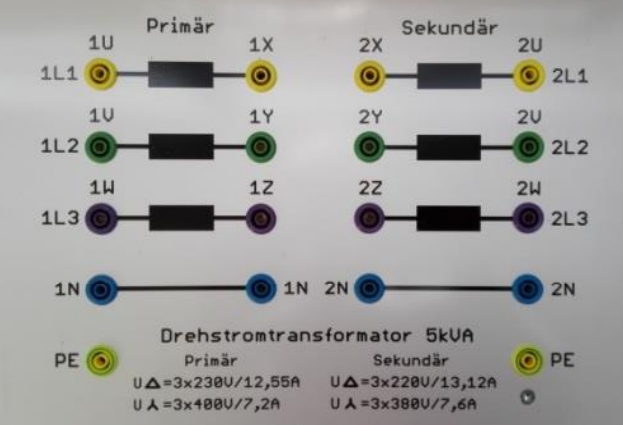
\includegraphics[width=0.75\textwidth]{img/3.1.2.1.png}
          \end{center}
          \caption{Nennwerte des Drehstromtransformators}\label{img:3.1.2.1}
        \end{figure}
        \begin{align*}
          \text{Dreieckverschaltung Primärseite}   \\
          U_N & = 230\ V                           \\
          I_N & = 12,55\ A                         \\
          \text{Sternverschaltung Primärseite}     \\
          U_N & = 400\ V                           \\
          I_N & = 7,2\ A                           \\
          \\
          \text{Dreieckverschaltung Sekundärseite} \\
          U_N & = 220\ V                           \\
          I_N & = 13,12\ A                         \\
          \text{Sternverschaltung Sekundärseite}   \\
          U_N & = 380\ V                           \\
          I_N & = 7,6\ A                           \\
        \end{align*}
        \pagebreak[2]
  \item Messen Sie bei primärseitigem Nennstrom (Kurzschlussstrom) die
        Kurzschlussspannung $U_K$ und den sekundären Kurzschlussstrom $I_2k$ aller drei
        Phasen sowie die zugehörigen Phasenwinkel. Beziehen Sie die Winkel auf der
        Primärseite auf $U_{12}$ der Primärseite. Auf der Sekundärseite messen Sie den
        Winkel zwischen $\underline U_{12}$ und $\underline I_1$ bezogen auf
        $\underline U_{12}$.

        \begin{table}[h!]
          \caption{Messwerte der Eingangsseite Yy0 Kurzschlussversuch}
          \centering
          \begin{tabular}{lllll}
            \\ \hline
            Phasen     & $\underline{U}$ in $[V]$ & $\varphi_{U}$ in $[^\circ]$ & $\underline{I}$ in $[A]$ & $\varphi_{I}$ in $[^\circ]$ \\ \hline
            $L1$       & $13$                     & $0$                         & $7,3$                    & $-52$                       \\
            $L2$       & $12$                     & $-121$                      & $7,3$                    & $-175$                      \\
            $L3$       & $12$                     & $121$                       & $7,0$                    & $65$                        \\ \hline
            Mittelwert & $12,300$                 & $0,000$                     & $7,200$                  & $-54,000$                   \\ \hline\hline
          \end{tabular}
        \end{table}
        \begin{table}[h!]
          \centering
          \caption{Messwerte der Ausgangsseite Yy0 Kurzschlussversuch}
          \begin{tabular}{lllll}
            \\ \hline
            Phasen     & $\underline{U}$ in $[V]$ & $\varphi_{U}$ in $[^\circ]$ & $\underline{I}$ in $[A]$ & $\varphi_{I}$ in $[^\circ]$ \\ \hline
            $L1$       & $0$                      & $0$                         & $7,4$                    & $-50$                       \\
            $L2$       & $0$                      & $0$                         & $7,5$                    & $-50$                       \\
            $L3$       & $0$                      & $0$                         & $7,0$                    & $-50$                       \\ \hline
            Mittelwert & $0,000$                  & $0,000$                     & $7,300$                  & $-50,000$                   \\ \hline\hline
          \end{tabular}
        \end{table}
\end{enumerate}

\subsection{Messungen bei symmetrischer Drehstromlast auf der Sekundärseite }
Belasten Sie den Transformator mit der ohmsch-induktiven Last nach Bild 11.\\
Bitte achten Sie auf den Nennstrom! ($U_{12} = 400\ V$ primärseitig). \\
Verwenden Sie zur Strommessung analoge und zur Spannungsmessung digitale
Messgeräte.
\begin{enumerate}[label=\alph*)]
  \item Dürfen Sie diese Last mit dem Transformator betreiben? Begründen Sie!\\ \ \\
        Die Verbindung der Last mit dem Transformator ist grundsätzlich möglich, da der
        Transformator in der Lage ist, den maximalen Strom, d.h., den Nennstrom von
        7,6A, zu liefern. Jedoch ist anzumerken, dass die Last möglicherweise nicht im
        Einklang mit den Nennwerten betrieben wird, denn der Nennbetrieb der Last liegt
        bei 9 A. Diese Konfiguration ist aus mehreren Gründen nicht empfehlenswert.\\ \
        \\

        Erstens führt der Betrieb des Transformators nahe der maximalen
        Belastungsgrenze zu einem erhöhten thermischen Stress und einer potenziellen
        Reduzierung der Lebensdauer des Transformators.\\ \ \\

        Zweitens ist zu beachten, dass die Last möglicherweise nicht mit den Nennwerten
        betrieben werden kann, dies könnte zu einer instabilen Betriebssituation
        führen, die nicht nur die Funktionalität der Last beeinträchtigt, sondern auch
        zu weiteren Schäden an anderen elektrischen Komponenten führen kann.\\ \ \\

        Insgesamt ist die vorgeschlagene Konfiguration nicht optimal, da sie das
        Potenzial für eine verkürzte Lebensdauer des Transformators und eine
        unsachgemäße Betriebsweise der Last birgt. Es wird empfohlen, alternative
        Konfigurationen zu prüfen, um eine effiziente und sichere elektrische
        Energieübertragung zu gewährleisten.\\ \ \\
\end{enumerate}
\pagebreak
\textbf{Schaltgruppe $Yy0$}
\begin{enumerate}[label=\alph*)]
  \setcounter{enumi}{1}
  \item Messen Sie alle Effektivwerte der Außenleiterspannungen und der
        Außenleiterströme auf der Primär- und Sekundärseite sowie alle zugehörigen
        Phasenwinkel. Beziehen Sie die Winkel auf der Primärseite auf $\underline
          U_{12}$ der Primärseite. Auf der Sekundärseite messen Sie den Winkel zwischen
        $\underline U_{12}$ und $\underline I_1$ bezogen auf $\underline U_{12}$.
        Messen Sie ebenfalls den Winkel zwischen den beiden Spannungen $\underline
          U_{12}$ auf der Primär- und der Sekundärseite.

        \begin{table}[h!]
          \caption{Messwerte der Eingangsseite Yy0 Symmetrischelast}
          \centering
          \begin{tabular}{lllll}
            \\ \hline
            Phasen     & $\underline{U}$ in $[V]$ & $\varphi_{U}$ in $[^\circ]$ & $\underline{I}$ in $[A]$ & $\varphi_{I}$ in $[^\circ]$ \\ \hline
            $L1$       & $378$                    & $0$                         & $7$                      & $-65$                       \\
            $L2$       & $371$                    & $-120$                      & $7$                      & $172$                       \\
            $L3$       & $372$                    & $120$                       & $7$                      & $53$                        \\ \hline
            Mittelwert & $373,667$                & $0,000$                     & $7,000$                  & $53,333$                    \\ \hline\hline
          \end{tabular}
        \end{table}
        \begin{table}[h!]
          \centering
          \caption{Messwerte der Ausgangsseite Yy0 Symmetrischelast}
          \begin{tabular}{lllll}
            \\ \hline
            Phasen     & $\underline{U}$ in $[V]$ & $\varphi_{U}$ in $[^\circ]$ & $\underline{I}$ in $[A]$ & $\varphi_{I}$ in $[^\circ]$ \\ \hline
            $L1$       & $357$                    & $0$                         & $7,0$                    & $-64$                       \\
            $L2$       & $347$                    & $120$                       & $7,0$                    & $-64$                       \\
            $L3$       & $358$                    & $-120$                      & $6,7$                    & $-64$                       \\ \hline
            Mittelwert & $354,000$                & $0,000$                     & $6,900$                  & $-64,000$                   \\ \hline\hline
          \end{tabular}
        \end{table}
        \pagebreak
\end{enumerate}
\textbf{Schaltgruppe $Dy5$}
\begin{enumerate}[label=\alph*)]
  \setcounter{enumi}{2}
  \item Messen Sie alle Effektivwerte der Außenleiterspannungen und der
        Außenleiterströme auf der Primär- und Sekundärseite sowie alle zugehörigen
        Phasenwinkel. Beziehen Sie die Winkel auf der Primärseite auf $\underline
          U_{12}$ der Primärseite. Auf der Sekundärseite messen Sie den Winkel zwischen
        $\underline U_{12}$ und $\underline I_1$ bezogen auf $\underline U_{12}$.
        Messen Sie ebenfalls den Winkel zwischen den beiden Spannungen $\underline
          U_{12}$ auf der Primär- und der Sekundärseite.

        \begin{table}[h!]
          \caption{Messwerte der Eingangsseite Dy5 Symmetrischelast}
          \centering
          \begin{tabular}{lllll}
            \\ \hline
            Phasen     & $\underline{U}$ in $[V]$ & $\varphi_{U}$ in $[^\circ]$ & $\underline{I}$ in $[A]$ & $\varphi_{I}$ in $[^\circ]$ \\ \hline
            $L1$       & $204$                    & $0$                         & $11$                     & $-65$                       \\
            $L2$       & $187$                    & $-120$                      & $11$                     & $170$                       \\
            $L3$       & $202$                    & $120$                       & $11$                     & $58$                        \\ \hline
            Mittelwert & $197,667$                & $0,000$                     & $11,100$                 & $54,333$                    \\ \hline\hline
          \end{tabular}
        \end{table}
        \begin{table}[h!]
          \centering
          \caption{Messwerte der Ausgangsseite Dy5 Symmetrischelast}
          \begin{tabular}{lllll}
            \\ \hline
            Phasen     & $\underline{U}$ in $[V]$ & $\varphi_{U}$ in $[^\circ]$ & $\underline{I}$ in $[A]$ & $\varphi_{I}$ in $[^\circ]$ \\ \hline
            $L1$       & $357$                    & $-152$                      & $7$                      & $-65$                       \\
            $L2$       & $347$                    & $94$                        & $6$                      & $-65$                       \\
            $L3$       & $358$                    & $-30$                       & $6$                      & $-65$                       \\ \hline
            Mittelwert & $354,000$                & $-29,333$                   & $6,300$                  & $-65,000$                   \\ \hline\hline
          \end{tabular}
        \end{table}
\end{enumerate}
\textbf{Die Primärseite bitte am Ende der Messung wieder in Stern verschalten! }
